\documentclass[a4paper,english, oneside, 12pt]{memoir} %kan laves til twoside
\chapterstyle{southall}
\usepackage[T1]{fontenc}
\usepackage[applemac]{inputenc}
\usepackage[english]{babel}
\usepackage{amsmath,amssymb,amsthm}
\numberwithin{equation}{section} 
\usepackage{booktabs,dcolumn,cellspace}
\usepackage{graphicx} %[pdftex]
\usepackage{wrapfig}
\usepackage{placeins} %float barrier
\usepackage[margin=3cm]{geometry} 
\setsecnumdepth{subsubsection}
\setcounter{tocdepth}{2}
\linespread{1.0}
\usepackage{array,booktabs}
\usepackage{caption}
\usepackage{subfig}
\usepackage{lscape}
\usepackage{array}
\usepackage{pbox}
\usepackage{lastpage}
%\usepackage{rotfloat}
\usepackage{multirow}
\usepackage{color}
\usepackage{relsize} 
\usepackage{fancyvrb}
\usepackage{tabularx}
%\usepackage{microtype}
\usepackage{rotating}
\usepackage{framed}
\usepackage{longtable}
\setlength{\parindent}{0pt}
\nonzeroparskip
\usepackage{lipsum}
\usepackage{listings}
\usepackage{algpseudocode}
\usepackage{textcomp}
\usepackage{hyperref}
\hypersetup{linktocpage}
\hypersetup{colorlinks,citecolor=red,filecolor=blue,linkcolor=red,urlcolor=blue}
\captionsetup[subfigure]{margin=10pt, parskip=0pt,hangindent=0pt, indention=0pt, singlelinecheck=true} 
\captionsetup[figure]{format=hang,justification=raggedright} %ndrer p caption pakken
\captionsetup{format=hang,justification=raggedright} %ndrer p caption pakken
\captionsetup[figure]{font={footnotesize,sf},labelfont=bf, singlelinecheck=1, width=0.85\textwidth}
\captionsetup[figure]{labelfont={bf,small},textfont={small}}
\captionsetup[subfloat]{labelfont={bf,small},textfont={small},
subrefformat=parens}
\usepackage{lineno}
\usepackage{minted}
\providecommand{\inlinecode}[1]{\texttt{\allowbreak#1}}
\providecommand{\todo}[1]{\addcontentsline{tdo}{todo}{\protect{#1}}\marginpar{\textcolor{red}{#1}}}
\newcommand{\tab}[1]{\hspace{.2\textwidth}\rlap{#1}}
\newcommand{\myparagraph}[1]{\paragraph{#1}\mbox{}\\}
\definecolor{listinggray}{gray}{0.9}
\definecolor{lbcolor}{rgb}{0.9,0.9,0.9}
\lstset{
  backgroundcolor=\color{lbcolor},
  tabsize=4,
  rulecolor=,
  language=matlab,
  basicstyle=\scriptsize,
  upquote=true,
  aboveskip={1.5\baselineskip},
  columns=fixed,
  showstringspaces=false,
  extendedchars=true,
  breaklines=true,
  prebreak = \raisebox{0ex}[0ex][0ex]{\ensuremath{\hookleftarrow}},
  frame=single,
  showtabs=false,
  showspaces=false,
  showstringspaces=false,
  identifierstyle=\ttfamily,
  keywordstyle=\color[rgb]{0,0,1},
  commentstyle=\color[rgb]{0.133,0.545,0.133},
  stringstyle=\color[rgb]{0.627,0.126,0.941},
}

\makepagestyle{plain}
\makeevenfoot{plain}{}{\thepage\ of \pageref*{LastPage}}{}
\makeoddfoot{plain}{}{\thepage\ of \pageref*{LastPage}}{}


\renewcommand\chapterheadstart{\vspace*{1 pt}}
\renewcommand\listingscaption{Example}
\def\listingautorefname{example}
\renewcommand\figureautorefname{figure}

\pagestyle{plain}


\begin{document}

\frontmatter
\begin{titlingpage}

\centering \parindent=0pt
\newcommand{\HRule}{\rule{\textwidth}{1mm}}
\vspace*{\stretch{1}} \HRule\\[1cm]
\Huge\bfseries TAPY\\[0.7cm]
\large Type Analysis for Python \\[1cm]
\HRule\\[2cm] \large Jesper Lindstr\o m Nielsen - \textit{jesper.jln@gmail.com} \\
\large Christoffer Quist Adamsen - \textit{christofferqa@gmail.com} \\
\large Troels Leth Jensen - \textit{troelslethjensen@gmail.com} \\

\vspace*{2 cm}  \normalsize 

\begin{flushleft}
Aarhus University\\
May 3, 2013 \end{flushleft}




\end{titlingpage}

%\tableofcontents

\mainmatter
\chapter*{Abstract}
We present a proof of concept for doing type analysis for Python using the monotone framework. We present how some interesting language features are converted into control flow graphs (CFGs), and also how it is possible to dynamically extend a CFG with calls to the so-called magic methods during the analysis, in order to minimize the total CFG in which the analysis works on. Finally, we show that our type analyzer is able to analyze small programs that involves non-trivial language features that distinguishes Python from other dynamic languages, e.g. JavaScript.
\chapter{Introduction}
Python is a dynamically typed, general purpose programming language that supports both object-oriented, imperative and functional programming styles. Python exploits a lot of its funtionality through Magic Methods (implicit method and function calls), this makes it harder to predict the outcome of simple statements and expressions.  \\
Because of its dynamic nature and little tool support it can be difficult to develop and maintain larger programs. In this report we present our work towards developing a conservative type analysis for Python version 2.7 in Scala.
\chapter{Our Approach}

Our approach for this project is to use existing frameworks and techniques with proven qualities to analyse the Python source code, most notably the monotone framework. This chapter contains outlines of how these frameworks and techniques are adapted to fit the specific task.

\section{Monotone framework implementation}

To get started an implementation of the monotone framework that is decoupled from the actual analysis was made. This implementation counts commonly used lattice structures, the worklist algorithm, a graph structure and an analysis interface (or trait in scala-lingo).

\subsection{Lattices}
In order to make our lives easier when constructing the actual analysis lattice, we have implemented several common lattice structures as type generic classes. These common lattice structures include, among others, a map and product lattice. In this section we will briefly go over the implementation decisions made for these structures.

Using classic object-oriented programming principles each of these compound structures decide the ordering of their elements by delegating to the underlying lattices in a point wise fashion, e.g. the product lattice has two underlying lattices, one for each element and thus the ordering is decided by comparing the first element in the pair in the context of the first lattice and similarly for the second element.

The map lattice has received a couple of changes from the naive implementation to make it usable in more cases. The first change was to interpret an unbound key value, $k$, to be a mapping from $k$ to the bottom element of the underlying lattice. In some use cases, such as a functional approach to intraprocedural static analysis, the map lattice will have a huge amount of keys. Requiring all of these to be bound to some value in the map is superfluous. This invariant is hidden completely in the lattice class because you can't manipulate the lattice element directly, so when trying to lookup an unbound key, the lattice simply constructs a fresh bottom value.

Since we now have a way to avoid binding every value from the key set, we are also able to change the constructor from the straightforward approach \inlinecode{k: Set[T], v: Lattice[S]} into a more general \inlinecode{k: T, v: Lattice[S]} (where \inlinecode{S} and \inlinecode{T} are type arguments). The straightforward approach has to compute the entire key set before you are able to instantiate the map lattice, but since the key set in itself might be exponentially large that wouldn't be practical. The downside to this change is, that since the map lattice has no way to know the intended key set, there is no way to construct the top element of the lattice.

% The top element of the lattice is useful for when you want to give up in the analysis, so to fix we instrumented the map lattice with a new top element, in a similar fashion to how the sink lattice instruments the underlying lattice with a new bottom element.

\subsection{Constraints}

Being in a functional programming language an easy-to-work-with representation of the constraints is anonymous lambda functions with the type \inlinecode{E $\rightarrow$ E}, where \inlinecode{E} is the type of the elements in the analysis lattice. Each constraint captures the node it was made from in its closure, so it is able to lookup the needed information in the lattice element.

This approach follows the notation very nicely, and as such makes the implementation a simple task when the constraints have been formulated formally.

\subsection{Worklist}
Our worklist implementation hasn't seen any optimizations and is as such just the straightforward implementation. First it generates constraint functions for each of the nodes in the CFG, adding each node to a worklist as it goes along. It then starts recursion (Scala benefits from tail call optimization to prevent the stack from exploding) on the list, popping one node from the list at a time. When a node is popped the corresponding constraint function is applied to the solution. Using Scalas built-in structural equality, the result is compared to the input and if they differ all nodes that depends on the popped node are added to the worklist.

A simple optimization would be to focus on finding a fixed-point for a strongly connected component of the CFG before continuing with the strongly connected components that depend on it, as also explained in section 5.1 from Static Program Analysis \cite{sa}.

\section{The Analysis Lattice}
Inspired by TAJS \cite{tajs} we have constructed a lattice for abstract values, $Value$ (see \autoref{lattice:Value}), from which we build a lattice for abstract objects, $Object$ (see \autoref{lattice:Object}). These two lattices are the main building blocks for the lattice of abstract states, $State$ (see \autoref{lattice:State}). Our analysis lattice is the lattice which for each program point (i.e. for each CFG node) describes the abstract state of that program point. Furthermore the $Analysis$ lattice (see \autoref{lattice:Analysis}) describes the call graph of the CFG.

\newpage
\subsection{Abstract Values}
The lattice for abstract values follows below:

\begin{figure}[H]
\begin{eqnarray*}
Value = & Undefined \times None \times NotImplemented \times Ellipsis \\
        & \times Boolean \times Integer \times Float \times Long \\
        & \times Complex \times String \times P(ObjectLabel)
\end{eqnarray*}
\vspace{-15pt}
\caption{The $Value$ lattice.}
\label{lattice:Value}
\end{figure}

The $Value$ lattice is used to describe the abstract values of temporary variables, and attributes on objects. The $Undefined$, $NotImplemented$, $Ellipsis$ and $None$\footnote{\inlinecode{NotImplemented}, \inlinecode{Ellipsis} and \inlinecode{None} are examples of built-in constants. See \cite{pyref.constants} for a complete list of built-in constants in Python.} lattices all contain two nodes, top and bottom. $NotImplemented$ is a constant in Python which can be used when a function is not supported. $Ellipsis$ is another constant which represents \inlinecode{\dots} in Python; this constant can be used when indexing using intervals (also known as slicing). When a function does not contain a return statement, the constant \inlinecode{None} is returned by default, e.g.:

\begin{listing}[H]
	\begin{minted}[linenos]{python}
def a(): pass
a() is None # true
	\end{minted}
	\caption{Constant None}\label{code:NoneExample}
\end{listing}

Contrary to JavaScript, Python supports integers, floats, longs and complex numbers, so we have separate lattices for those. As lists in Python can only be indexed using integers our lattices does not have to keep track of whether a particular number is an unsigned integer or not, as the $Num$ lattice for TAJS does (page 8, \cite{tajs}). To TAJS it is crucial to have this distinction because the behavior of associative arrays are distinct based on whether an unsigned integer or not is used to index with. For the similar reason our $String$ lattice does not distinct between unsigned integer strings and arbitrary strings, as the $String$ lattice for TAJS does.

Note that $Complex = Float \times Float$, since a complex number in Python is represented using a float for the real and imaginary part, respectively \cite{pyref.stdtypes}. The $Integer$ lattice is defined here in \autoref{fig:latticeInteger}. The $Float$, $Long$ and $String$ lattices are defined in similar ways. Finally, a value can also be a pointer to an object on the heap, which we model in the $Value$ lattice by having a power set\footnote{All our power sets are ordered by subset inclusion.} of object labels, $P(ObjectLabel)$.

The notion of object labels will be described in \autoref{The Heap} about the heap.

\begin{figure}[H]
	\begin{center}
		\includegraphics[width=0.25\textwidth]{images/integer-lattice.png}
	\end{center}
	\vspace{-15pt}
	\caption{The integer lattice}
	\label{fig:latticeInteger}
\end{figure}



\subsection{Abstract State}
We use the following lattice to model abstract state:

\begin{figure}[H]
\begin{equation*}
State = Heap \times Stack
\end{equation*}
\vspace{-15pt}
\caption{The $State$ lattice.}
\label{lattice:State}
\end{figure}

Before we describe the $Heap$ (\autoref{The Heap}) and $Stack$ (\autoref{The Stack}) lattices, we need to look at the $Object$ lattice:

\begin{figure}[H]
\begin{equation*}
Object = (AttributeName \rightarrow Value \times Global) \times P(ObjectLabel^{*})
\end{equation*}
\vspace{-15pt}
\caption{The $Object$ lattice.}
\label{lattice:Object}
\end{figure}

Having made special lattices for the 'primitive' objects there is still a need to handle the more complex objects such as class instances and function objects. As with JavaScript you can augment objects with attributes at runtime, so the lattice needs to accommodate this dynamic behavior. We therefore use a map from attribute names to values. For some objects it is required to track the scope in which they were defined, to model the closure they are evaluated in. Additionally, variable scope objects will be modeled with abstract values of this type, and here the ability to mark variables as global is needed, indicating that writes to this variable should be done in the global variable scope object. Thus the object lattice is the product between object values and a static scope chain modeled as a list of object labels. The static scope chain is only present for function objects and describes the scope of the function at its declaration. It is used to properly update the scope chain when calling the function.

\newpage

\subsection{The Heap}
\label{The Heap}

\begin{figure}[H]
\begin{equation*}
Heap = (ObjectLabel \rightarrow Object)
\end{equation*}
\vspace{-15pt}
\caption{The $Heap$ lattice.}
\label{lattice:Heap}
\end{figure}

The heap is modeled by a map from object labels to object values. During the execution of a program there may be unbounded many objects on the heap, which we must approximate with a finite representation. We do this by using an object label for each allocation site, i.e. each node in the CFG that may create a new object on the heap. This is commonly known as the \textit{allocation-site abstraction} \cite{recency,aopas}, which we get back to in \autoref{section:Strong or weak}. Thus, our abstract heap lattice will only contain one object for each such allocation site.

As an illustrative example consider the following very simple program:

\begin{listing}[H]
	\begin{minted}[linenos]{python}
class C(): pass
x = []
for y in range(0,2):
  x.append(C())
x[0].a = 'a'
x[1].b = 'b'
	\end{minted}
	\caption{Imprecision introduced by allocation-site abstraction.}
\end{listing}

At runtime this example generates two different \inlinecode{C} objects with attributes \inlinecode{a} and \inlinecode{b}, respectively. Using the allocation-site abstraction only a single \inlinecode{C} object would be created on the abstract heap. As a consequence, when writing to the attribute \inlinecode{a} at line 5, this is in principle done on each object originating from the same allocation-site\footnote{In order to deal with this conservatively, it must of course be a weak update. We discuss strong and weak updates in \autoref{section:Strong or weak}.}. Thus an analysis for this code should conclude at the end that the attribute \inlinecode{a} of an object originating from line 4 might be undefined or \inlinecode{'a'} (similar for \inlinecode{b}).

As a side note we mention that the approach taken here is quite similar to the one taken in the Static Analysis course\footnote{See \url{http://cs.au.dk/SA}.}, where a couple of points-to analyses for Tiny Imperative Language (TIP) was described. There, \textit{Targets} was introduced as the possible set of allocations-sites, which for TIP is the pointer targets \inlinecode{malloc-i} for a given program (page 74, \cite{sa}).

In our type analyser we found it beneficial to distinguish between different types of object labels but still handle them in the same way in the heap. To achieve this we made several different subclasses to the object label, e.g. a function object label, which besides its name also holds a reference to the CFG node that is the entry node for that function.


\subsection{The Stack}
\label{The Stack}
The $Stack$ lattice is defined as:

\begin{figure}[H]
\begin{equation*}
Stack = (Register \rightarrow Value) \times P(ObjectLabel^{*})
\end{equation*}
\vspace{-15pt}
\caption{The $Stack$ lattice.}
\label{lattice:Stack}
\end{figure}

For each register, which can be thought of as a temporary variable, we specify the value of that particular register. Recall that we use registers in our intermediate representation, see \autoref{fig:callCfg} in \autoref{CFG calls} about CFG construction of function and method calls.

The power set $P(ObjectLabel^{*})$ specifies the objects on the dynamic scope chain $ObjectLabel^{*}$, i.e. the runtime stack. The head element in the scope chain determines which object on the heap, local variable writes should we written to. For instance we will have an object on the heap for each program, that models the module/top-level script environment \inlinecode{\_\_main\_\_} \cite{pyref.main} (this is what corresponds to the global object in JavaScript). Whenever an assignment to a variable occurs in the top-level scripting environment, e.g. \inlinecode{x=10}, the variable \inlinecode{x} is set as a attribute mapping to the integer 10 on the \inlinecode{\_\_main\_\_} object in the heap.

The dynamic scope chain is captured as the static scope chain whenever a class or function is declared. This new static scope chain is stored in the $Object$ lattice as seen in \autoref{lattice:Object}. The following example demonstrates this:

\begin{listing}[H]
	\begin{minted}[linenos]{python}
x = 10
def a():
  return x
a() # 10
x = 42
a() # 42
	\end{minted}
\caption{Scope example.}
\label{code:ScopeExample}
\end{listing}

For this example we will have the following objects on the abstract heap:

\begin{enumerate}
  \item The \inlinecode{\_\_main\_\_} object,
  \item The object of the function \inlinecode{a},
  \item The scope object of \inlinecode{a} (which is an object similar to the \inlinecode{\_\_main\_\_} object, i.e. an object where local variables are written onto).
\end{enumerate}

When calling the function the dynamic scope chain will be set to the static scope chain related to the function \inlinecode{a} in order to model Pythons static scoping. When the variable \inlinecode{x} is read, \inlinecode{x} is looked up in the scope chain; for this particular example \inlinecode{x} is found on the \inlinecode{\_\_main\_\_} object.

In the \autoref{Functions} we describe our work towards handling functions, this includes populating the call graph such that the CFG becomes interprocedural.

\begin{figure}[H]
\begin{eqnarray*}
CallGraph = & P(Node \times Node) \\
Analysis = & (Node \rightarrow State) \times CallGraph
\end{eqnarray*}
\vspace{-15pt}
\caption{The $CallGraph$ and $Analysis$ lattice.}
\label{lattice:Analysis}
\end{figure}
\chapter{The Control Flow Graph}
\label{chap:CFGConstruction}
In this section we give examples of how we inductively generate the control flow graph of some essential language features. 
During this we will present the control flow graph nodes that we use, together with their semantics.



\section{An example: For loops}
\label{sec:CFGConstructionLoops}
Loops in Python differs from loops in most other languages as both \inlinecode{for} and \inlinecode{while} loops have an \inlinecode{else} branch, as can be seen in example \ref{code:forExample}. The \inlinecode{else} branch is executed if the loop terminates normally, i.e. not using the \inlinecode{break} statement.

\begin{listing}[H]
  \begin{minted}[linenos]{python}
for x in [1,2,3]:
  if (x > 2):
    break
  print x
else:
  print "normal for termination"
  \end{minted}
  \caption{For loop example with an \inlinecode{else} block.}\label{code:forExample}
\end{listing}

First, the expression given to the for loop, \inlinecode{[1,2,3]}, is evaluated. This should result in an iterable object, such that an iterator object can be created. Now for each element of the iterator the body of the for loop is evaluated once.

To simulate the evaluation sequence of such a for loop in our CFG, we need to take a look at the iterator object: 
to get the next element from an iterator object the \inlinecode{next} method can be called. This method returns the next element until the iteration is done and finally raises a \inlinecode{StopIteration} exception.

The CFG our type analyzer generates for example \ref{code:forExample} can been seen in figure \ref{fig:forCfg}.

\begin{figure}{H}
  \begin{center}
    \includegraphics[width=0.8\textwidth]{images/for-example-cfg2.png}
  \end{center}
  \caption{Control Flow Graph for the for-loop example \ref{code:forExample}}
  \label{fig:forCfg}
\end{figure}

%\begin{wrapfigure}{r}{0.5\textwidth}
%  \vspace{-20pt}
%  \begin{center}
%    \includegraphics[width=0.48\textwidth]{images/while.png}
%  \end{center}
%  \vspace{-10pt}
%  \caption{Control Flow Graph for a while-loop}
%  \label{fig:whileCfg}
%  \vspace{-10pt}
%\end{wrapfigure}

%For a while loop we generate the control flow graph in figure \ref{fig:whileCfg}.



\section{Using registers for the intermediate representation}
\label{CFG calls}
Inspired from TAJS \cite{tajs}, Type Analyzer for JavaScript, we use registers in our intermediate representation to model that even simple expressions in Python is evaluated in several steps. To illustrate this consider the following line of code from example \ref{code:Features1}: \inlinecode{s1.addGrade('math', 10)}.

First the function \inlinecode{addGrade} is looked up in the class of \inlinecode{s1}. This is done in the CFG using \textit{ReadAttributeNode}, which holds a result register, a base register, i.e. the register where to find the object, and the name of the attribute to look up. Similar nodes include \textit{ReadVariableNode} and \textit{ReadIndexableNode}.

\begin{wrapfigure}{r}{0.5\textwidth}
	\vspace{-20pt}
	\begin{center}
		\includegraphics[width=0.48\textwidth]{images/Call-example.png}
	\end{center}
	\vspace{-10pt}
	\caption{Control Flow Graph for a call example}
	\label{fig:callCfg}
	\vspace{-10pt}
\end{wrapfigure}

Second, each argument given to the function is evaluated, and finally the actual call is done. Calls in the control flow graph is modeled using the \textit{CallNode}, which holds a function register and a list of argument registers, and \textit{AfterCallNode}, which holds a result register.

Thus the expression \inlinecode{s1.addGrade('math', 10)} will result in the control flow graph found in figure \ref{fig:callCfg} 
(where the numbers to the left represent the result registers of the nodes).

So far we have primarily been concerned with putting constants into registers and reading e.g. variables. In order to support writing we have three different nodes: \textit{WriteVariableNode}, \textit{WriteAttributeNode}, and \textit{WriteIndexableNode}. Besides holding a value register, i.e. the register where to find the value being written, \textit{WriteVariableNode} contains the name of the variable being written to, \textit{WriteAttributeNode} contains a base register and the attribute being written to, and \textit{WriteIndexableNode} contains a base and attribute register (the latter has a register for the attribute because it is not constant, for instance we could write something like the following: \inlinecode{dict[getKey()] = aValue}, whereas attribute in \inlinecode{obj.attribute = aValue} must be a string).



\section{Magic methods}
The so-called magic methods can be thought of as hooks, which allow the programmer to get to execute code at e.g. attribute access. This is something that cannot be done in e.g. JavaScript.

From a static analysis point of view some of these magic methods are less interesting, as e.g. \inlinecode{\_\_init\_\_}. This particular magic method just corresponds to a constructor.

Two very interesting magic methods, however, are \inlinecode{\_\_getattribute\_\_} and \inlinecode{\_\_getattr\_\_}. These are particular interesting because each time an attribute \inlinecode{a} is read from a class object \inlinecode{x}, the following happens:

The magic method \inlinecode{\_\_getattribute\_\_} is looked up on \inlinecode{x}. If it is defined, the method is called with the instance, \inlinecode{x}, and the attribute name \inlinecode{a}. It is now up to the supplied method to return the correct value\inlinecode{For instance the implementation of \inlinecode{\_\_getattribute\_\_} could just return a constant, which would cause every attribute access to result in that particular constant.}. If the implementation of \inlinecode{\_\_getattribute\_\_} happens to raise an \inlinecode{AttributeError}, \inlinecode{\_\_getattr\_\_} is called. Otherwise if \inlinecode{\_\_getattribute\_\_} is not defined, the attribute is looked up on the instance. If the attribute is present on the instance it is returned, otherwise an \inlinecode{AttributeError} is raised and the magic method \inlinecode{\_\_getattr\_\_} is called (at least if it is defined).

The following pseudo code should illustrate this:

\begin{listing}[H]
  \begin{minted}[linenos]{python}
def readAttribute(x, a):
  __getattribute__ = lookup(x, '__getattribute__')
  __getattr__ = lookup(x, '__getattr__')

  try:
    if isset(__getattribute__):
      # __getattribute__ is called if defined
      return __getattribute__(x, a)
    else:
      return getattr(x, a)
  except AttributeError as e:
    if isset(__getattr__):
      # __getattr__ called in case of an AttributeError
      return __getattr__(x, a)
    else
      raise e
  \end{minted}
\end{listing}

Thus, the magic method \inlinecode{\_\_getattribute\_\_} can be used to supply a custom attribute lookup function, and \inlinecode{\_\_getattr\_\_} can be used to supply a fallback function in case of a bad attribute access. Note also that the \inlinecode{\_\_getattribute\_\_} can not be thought of as being equivalent (or nearly equivalent) to getters in e.g. ECMAScript 5 and C\#: In Python one single method is supplied, not one for each attribute (or property and field for ECMAScript 5, respectively C\#).

As mentioned in the introduction we have only aimed to support \inlinecode{\_\_getattr\_\_} in our type analyzer, due to the limited time of our project. However, in order to determine that we wanted to support \inlinecode{\_\_getattr\_\_} and not \inlinecode{\_\_getattribute\_\_}, we looked at the use of these magic methods in some larger Python projects. In Django 1.5.1\footnote{See \url{http://www.djangoproject.com/}.}, a high-level web framework, we found that \inlinecode{\_\_getattribute\_\_} was not used at all. However, \inlinecode{\_\_getattr\_\_} is used 14 times and therefore seems more useful to support if the choice stands between the two of them. Of course 14 usages is not much for a web framework on approximately 200.000 lines of code, but it is still essential to handle in order to be able to statically analyze Python programs.

\subsection{Transforming the CFG}
\label{Magic methods transformation}
Since each single attribute access possibly involves method calls, we normalize the CFG in order to reflect this. More concretely, we normalize each node in the CFG of the following form: \inlinecode{<res>=ReadAttribute(<base>,prop)}, into the following CFG piece:

\begin{listing}[H]
  \begin{center}
    \includegraphics[width=0.9\textwidth]{images/readproperty.png}
  \end{center}
  \vspace{-10pt}
  \caption{The normalization of a read attribute node.}
  \label{fig:MagicMethods1}
\end{listing}

As can be seen from the normalized CFG of read attribute nodes the only challenge there is in order for our analysis to handle the magic method \inlinecode{\_\_getattr\_\_}, is that we need to handle exceptions in our analysis. We return to this in the following section. First, we want to note that if an attribute is \textit{definitely} set on an instance object, \inlinecode{\_\_getattr\_\_} is never called when reading that particular attribute. This is the case as there won't be any flow across the exception edge in the figure above, because the \inlinecode{ReadAttributeNode} will always succeed in reading the attribute and therefore not raise any \inlinecode{AttributeError}. When we can't conclude that an attribute is definitely available (e.g. as in the example below), we must of course normalize the read attribute node.

\begin{listing}[H]
  \begin{minted}[linenos]{python}
class C():
  if (trickyComputation()):
    C.a = 42
  def __getattr__(self, name):
    return "<bad attribute access>"
x = C()
y = x.a # __getattr__ will be called if trickyComputation() returned false
  \end{minted}
  \caption{A simple example of when it will be possible to conclude that \inlinecode{\_\_getattr\_\_} will never be called even though \inlinecode{\_\_getattribute\_\_} is defined.}
  \label{code:MagicMethods2}
\end{listing}

Thus the type analyzer can be improved such that it only normalizes read attribute nodes if the attribute being read may not be defined (resulting in possibly $12 * \#\texttt{read attribute nodes}$ nodes less in the CFG). This is in fact what our implementation does. In order to obtain this we have provided the analysis with a hook from the work list algorithm, such that our type analyzer can modify the control flow graph during the analysis. When doing this, each newly added node to the CFG must of course be added to the work list.

It is important to note however, that not supporting \inlinecode{\_\_getattribute\_\_} simplifies the task a bit. Recall that we don't need to normalize read attribute nodes as long the attribute being read is definitely set. This is not the case if we took the magic method \inlinecode{\_\_getattribute\_\_} into account, as it might itself raise an \inlinecode{AttributeError} (causing \inlinecode{\_\_getattr\_\_} to be called)! Thus a type analysis that also supports \inlinecode{\_\_getattribute\_\_} would for a start actually have to normalize all read attribute nodes where an attribute is dereferenced from an instance that belongs from a class where \inlinecode{\_\_getattribute\_\_} is defined. In some cases it might of course be possible to conclude that the particular implementation of \inlinecode{\_\_getattribute\_\_} will never raise an \inlinecode{AttributeError}, e.g. when the implementation just returns a constant (see the example below), in which the type analysis of course don't need to normalize the read property node.

\begin{listing}[H]
  \begin{minted}[linenos]{python}
class C(object):
  def __getattribute__(self, name):
    return 42
  def __getattr__(self, name):
    return "<bad attribute access>"
x = C()
y = x.a # no attribute access will result in __getattr__ being called
  \end{minted}
  \caption{A simple example of when it will be possible to conclude that \inlinecode{\_\_getattr\_\_} will never be called even though \inlinecode{\_\_getattribute\_\_} is defined.}
  \label{code:MagicMethods2}
\end{listing}









\section{Handling exceptions}
In order to handle the flow caused by exceptions we use two different kinds of edges in the control flow graph. 
A solid edge indicates normal flow, and a dashed edge indicates exception flow. 

In Python exceptions can be caught using a try-except-else-finally block. An except block can be annotated with a number of types, 
and each try-except-else-finally block may contain an arbitrary number of except blocks. As usual, the else block is entered in case of a normal exit, 
i.e. when no exceptions were raised inside the try block.

The AST provided by the Jython parser has been normalized from a try-except-else-finally block into a try-finally block, 
which contains a try-except-else block in its try block.

For instance the code in the first example \ref{code:tryExceptBefore} below is transformed into the code in the next example \ref{code:tryExceptAfter}:

\begin{listing}[H]
	\begin{minted}[linenos]{python}
try:
  <try-stms>
except Foo:
  <except-foo-stms>
except:
  <except-stms>
else: 
  <else>
finally:
  <finally>
	\end{minted}
	\caption{A try-except-else-finally example before convertion}\label{code:tryExceptBefore}
\end{listing}

\begin{listing}[H]
	\begin{minted}[linenos]{python}
try: 
  try:
    <try-stms>
  except Foo:
    <except-foo-stms>
  except:
    <except-stms>
  else:
    <else-stms>
finally:
  <finally-stms>
	\end{minted}
	\caption{A try-except-else-finally example after convertion}\label{code:tryExceptAfter}
\end{listing}

\begin{sloppypar}
  Inductively, CFG's for the statement lists <\inlinecode{try-stms}> (\textit{CFG$_{\textit{try}}$}), 
  <\inlinecode{except-foo-stms}> (\textit{CFG$_{\textit{except-foo}}$}), <\inlinecode{except-stms}> (\textit{CFG$_{\textit{except}}$}), 
  <\inlinecode{else-stms}> (\textit{CFG$_{\textit{else}}$}), and <\inlinecode{finally-stms}> are created. 
\end{sloppypar}

The CFG for the finally block is then cloned into three duplicates (\textit{CFG$_{\textit{finally-normal}}$}, 
\textit{CFG$_{\textit{finally-handled-exc}}$}, \textit{CFG$_{\textit{finally-unhandled-exc}}$}). The purpose is to have one finally block for each of the following cases: 

\begin{enumerate}
  \item when no exceptions occur during the try block,
  \item when an exception is raised and caught by one of the surrounding except blocks, and no exception is raised from inside that except block, and
  \item when an exception is raised but not caught, which is the case when 
    a) an exception is raised from the try block and no except blocks handles this particular exception, 
    b) an except block catches an exception raised by the try block, but then raises a new exception on its own.
\end{enumerate}

\begin{sloppypar}
  In particular, it is important that the finally block for handling case (3), i.e. \textit{CFG$_{\textit{finally-unhandled-exc}}$}, 
  is not connected to the exit node of the try-except-else-finally block. Instead, it should be connected to its nearest surrounding except block (if any), 
  or no except block at all (indicating that the program crashes with a runtime error because of an unhandled exception).
\end{sloppypar}

In the following sections we present the way we generate the CFG of a try-except-else-finally block.



\subsection{The try block}
Each node in \textit{CFG$_{\textit{try}}$} (that does not already have an outgoing exception edge) is connected using an exception edge to the entry node of the first except block (*), in this case the entry node of \textit{CFG$_{\textit{except-foo}}$}. We do not add exception edges to nodes that already have an exception edges, because this would be a loss of information: the control flow always goes to the nearest enclosing except block in case of exceptions. \\
The above models that if an exception occurs during evaluation of one of the statements in a try block, then the control flow will proceed from the first except block. \\
If there is no except blocks, each node should instead be connected using an exception edge to the entry node of its nearest surrounding except or finally block (specifically \textit{CFG$_{\textit{finally-unhandled-exc}}$}). However, we don't add any exception edges here; these will be added inductively because of (*) in case there are any surrounding except or finally blocks.

\begin{wrapfigure}{r}{0.5\textwidth}
  \vspace{-20pt}
  \begin{center}
    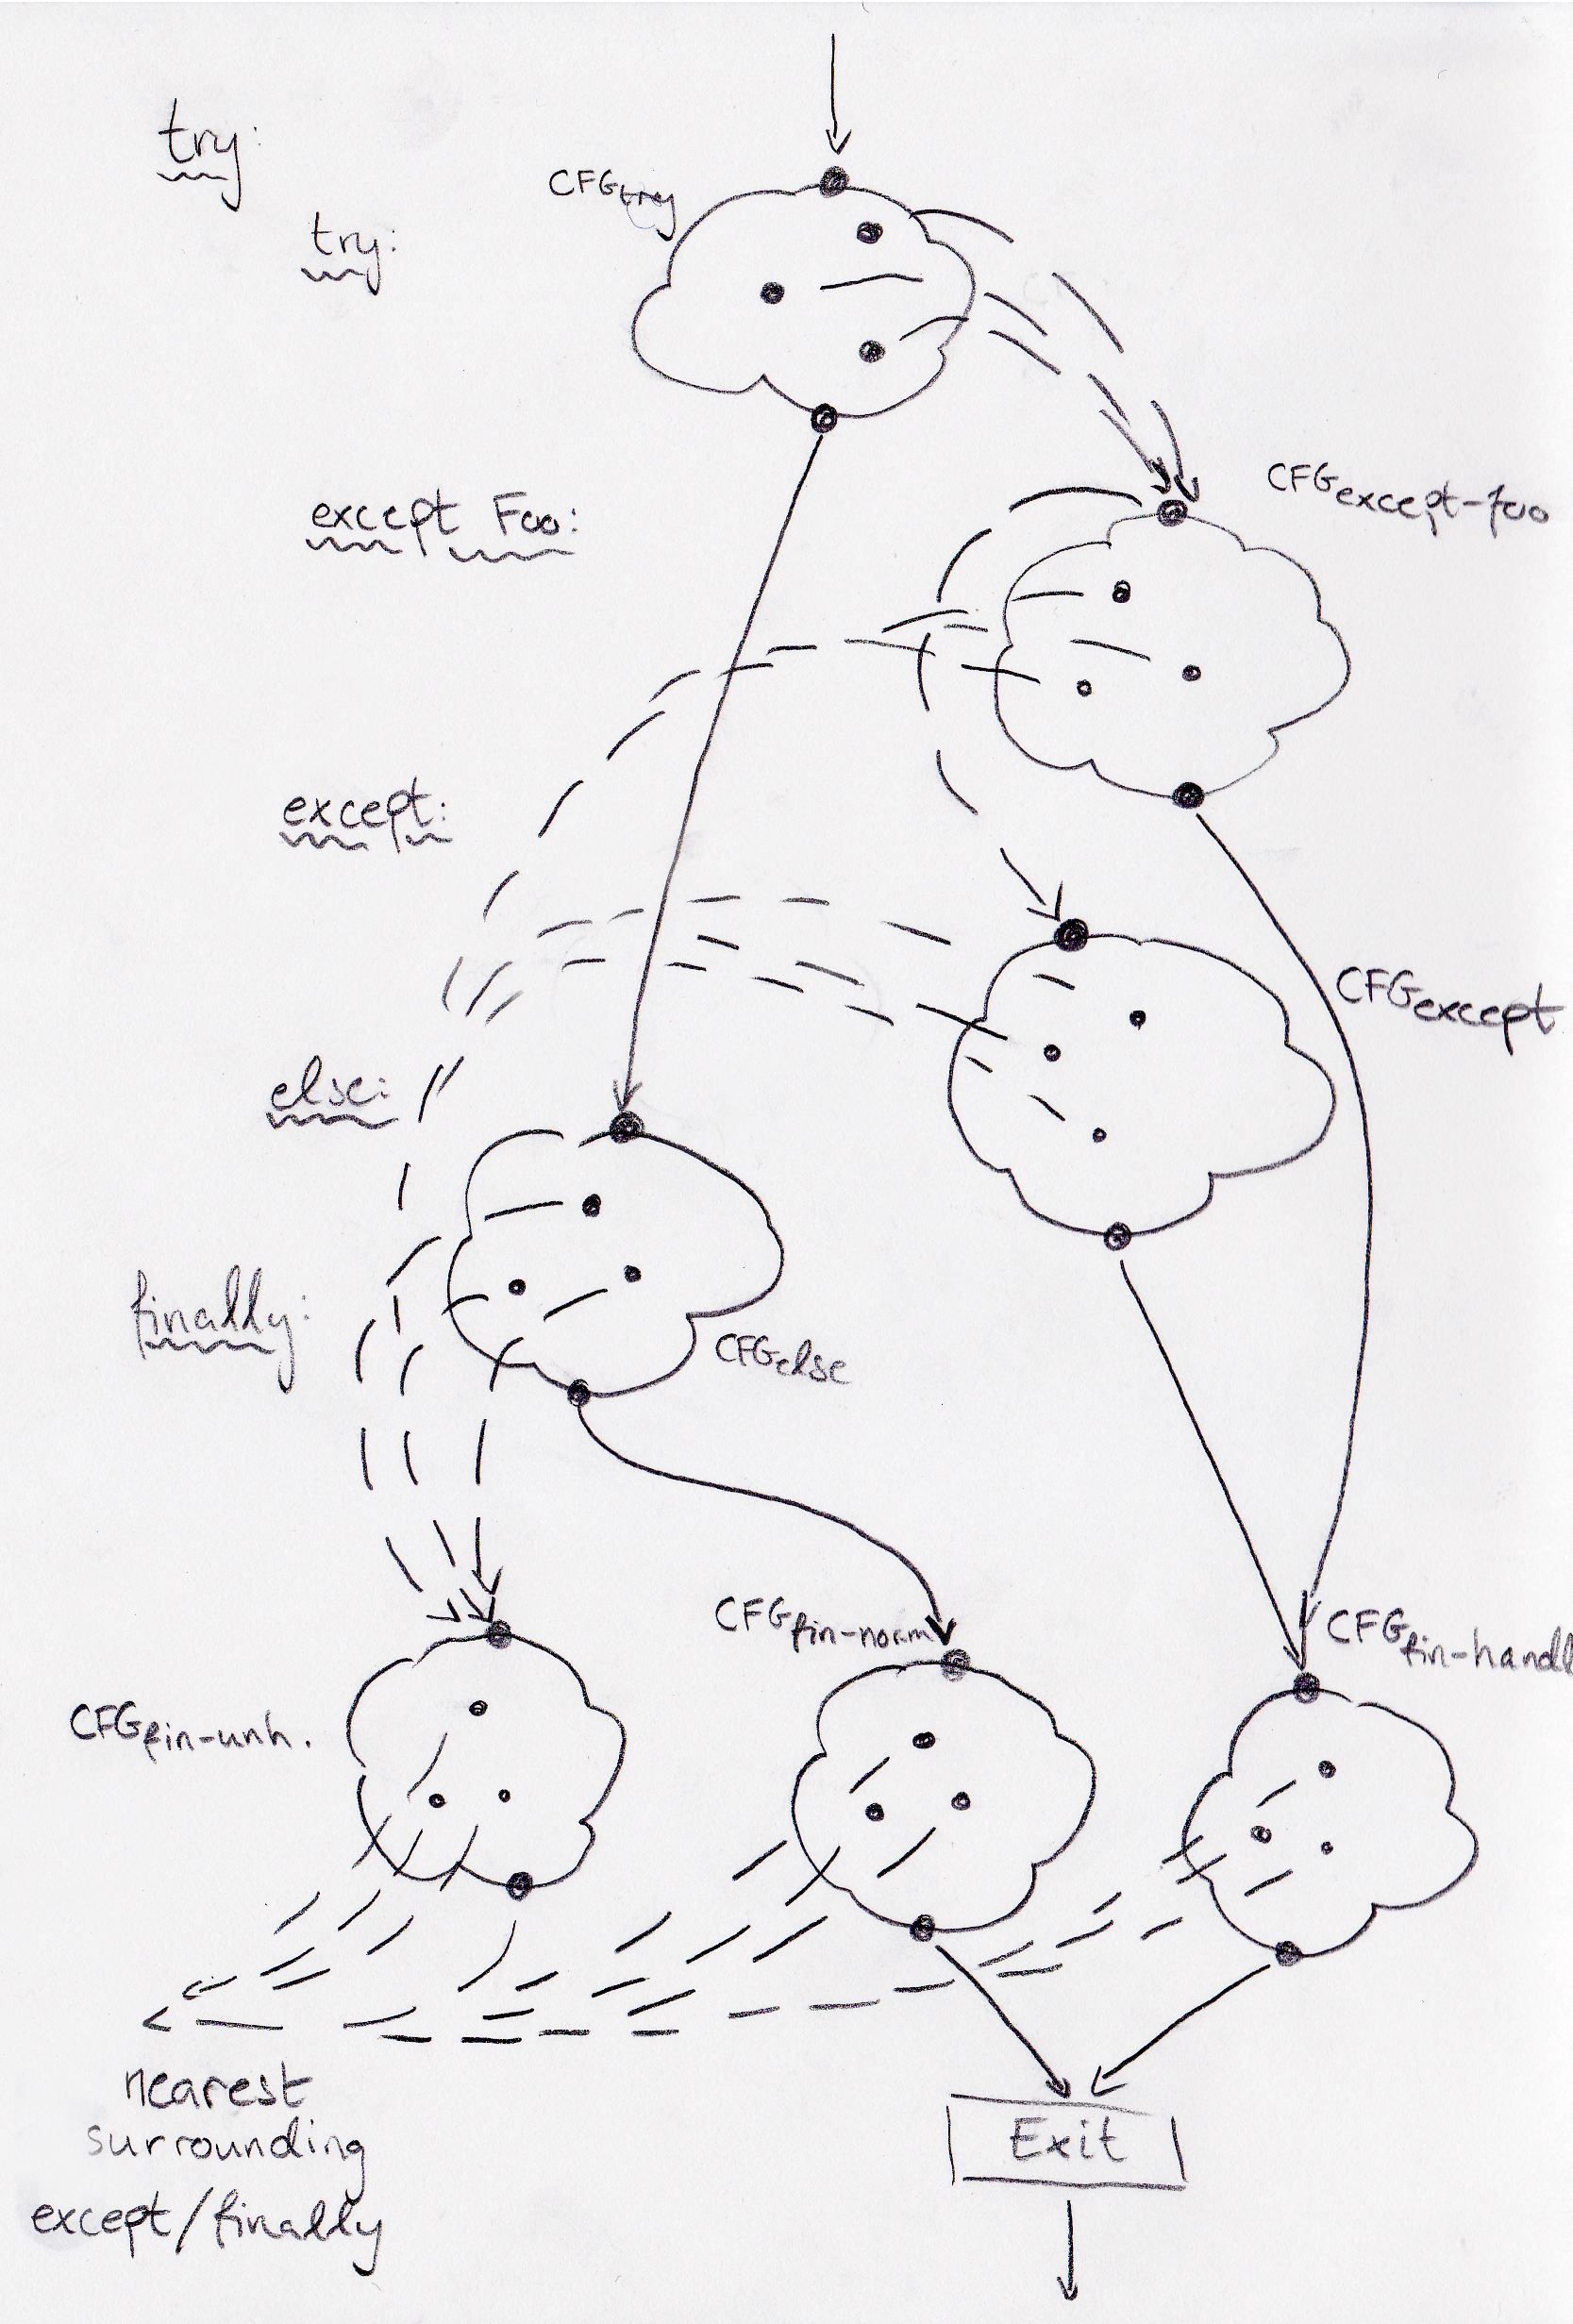
\includegraphics[width=0.48\textwidth]{images/Try-except-else-finally.png}
  \end{center}
  \vspace{-10pt}
  \caption{Control Flow Graph for try try-except example \ref{code:tryExceptAfter}}
  \label{fig:tryExceptCfg}
  \vspace{-10pt}
\end{wrapfigure}



\subsection{The except block}
The entry node of each except block is connected using an exception edge to the entry node of the next except block (except for the last block, of course). 
Thus we make an exception edge from the entry node of \textit{CFG$_{\textit{except-foo}}$} to the entry node of \textit{CFG$_{\textit{except}}$}.

We do this because the first except block might not catch the exception (because of the type restrictions), 
in which the control flow proceeds at the next except block.

Furthermore, each node inside the except block should be connected using an exception edge to the entry node
 of its nearest surrounding except or finally block (specifically \textit{CFG$_{\textit{finally-unhandled-exc}}$}). As above, this is handled inductively.

Finally, if an except block actually catches the exception, and no exceptions occur inside that except block, 
the control flow proceeds to the surrounding finally block (in this case, \textit{CFG$_{\textit{finally-handled-exc}}$}). 



\subsection{The else block}
If no exceptions occur, the else block should be evaluated. Thus we add a normal flow edge from the exit node of \textit{CFG$_{\textit{try}}$} 
to the entry node of \textit{CFG$_{\textit{else}}$}.

Since exceptions may result from evaluating the statements in the else block, each node in \textit{CFG$_{\textit{else}}$} 
should also be connected to the entry node of the nearest surrounding except or finally block (again, \textit{CFG$_{\textit{finally-unhandled-exc}}$}).

In case the evaluation of the statements in the else block does not raise any exceptions, 
the control flow proceeds either to the exit node of the whole try-except-else block, or in case there is a surrounding finally block, 
to the entry node of \textit{CFG$_{\textit{finally-normal}}$}.



\subsection{Global Statement}
At first glance the \inlinecode{global} statement in Python seems rater straightforward to analyze, but it has some interesting quirks that are not that intuitive, and thus deserves special handling. In this section we will go over these quirks and how this affected the analysis of this statement.

The statement allows for a function to declare an identifier to be considered global for the entirety of the function body. No matter where the global statement is stated within the function body it will take effect for the entire function body, even for statements that are stated before the global statement. It should also be noted that the statement doesn't have to be executed to take effect, so global statements in dead code also take effect.

When an identifier has declared global, all variable lookups (both reads and writes) on that identifier are done directly in the global scope (module level) without consideration for any scopes that might have been checked firsts under regular circumstances.

Since the \inlinecode{global} statement can only move a variable from the enclosing function scope to the global scope and to or from any scopes in between it is statically possible to determine the variable location in all cases, and thus we can make a strong update by marking the identifier as global. 

Due to the fact that the global statement takes effect no matter where it is in the function body, it courses problems for the join function since a situation where a variable X is marked as global in one state and not in the other can arise. In such a situation, the state where the variable is not marked as global is in principal incorrect, since the global statement changes the variable for the entire scope, so it has to do some fixing to change this. To avoid this problem a preprocessing step is introduced in which the CFG node corresponding to the \inlinecode{global} statement is moved such that it appears only before branching. That way the join function can stay the same.



\section{CFG construction of With statements}
With statements in Python are unlike With statements in JavaScript.\ They are usually used when you have object you need to "open" before you do some work and then "close" it in the end, this pattern is used a lot when working with I/O such as files or databases.\ An example of with statements can be seen in Listing \ref{code:withExample}.

\begin{listing}[H]
  \begin{minted}[linenos]{python}
with open('file.txt') as fh:
  print fh.read()
  \end{minted}
  \caption{With example reading a file}\label{code:withExample}
\end{listing}

The formal description of the With statement can be found in The Python Language Reference compound statement list\cite{pyref.compound} section 7.5, 
the highlights is that if there is an \inlinecode{as} part of your with statement the result of the method call to \inlinecode{\_\_enter\_\_} 
assigned to the variable in the with statement. If there is raised an exception during the execution of the body of the With statement it is 
passed as arguments to the method call \inlinecode{\_\_exit\_\_}, if the result of that call returns something which truth value is \inlinecode{True} 
the with statement just evaluates normally, If a truth value of \inlinecode{False} is returned the exception isn't caught. 
If no exceptions happens during execution the \inlinecode{\_\_exit\_\_} method is called, after the body of the With statement, 
where \inlinecode{None} is passed as arguments.
\chapter{Analysing Functions}
\label{Functions}
In this chapter we motivate why the analyser puts two objects on the abstract heap for each function declaration, as mentioned in \autoref{The Stack}. One being the function object, and the other being the function scope object. The function object is necessary as functions are themselves objects, just like in JavaScript. For instance we can set an attribute on a function object:

\begin{listing}[H]
	\begin{minted}[linenos]{python}
def foo(): pass
foo.attr = 42
	\end{minted}
\caption{Setting an attribute on a function object.}
\label{code:FunctionPropertyExample}
\end{listing}

%Another thing with regards to function objects on the heap, is that Python has a built in method \inlinecode{\_\_call\_\_} on each function. This method is a function wrapper of the function itself; calling it will result in calling the function itself. We therefore map the attribute \inlinecode{\_\_call\_\_} on the function object to its function wrapper object. The following illustrates how each newly declared function has this method:

%\begin{listing}[H]
%	\begin{minted}[linenos]{python}
%def a():
%	print "a"
%a() // "a"
%a.__call__ # <method-wrapper '__call__' of function object at ...> 
%a.__call__() # "a"
%	\end{minted}
%\caption{On a newly declared function the \_\_call\_\_ attribute is set to a built in method wrapper.}\label{code:printFunctionExample}
%\end{listing}

%It is important to distinguish between the object of the function, and the function object, since \inlinecode{\_\_call\_\_} is not just a reference to the object of the function, as illustrated below:

%\begin{listing}[H]
%	\begin{minted}[linenos]{python}
%def a(): 
%	pass
%
%# TypeError: 'method-wrapper' object has only read-only attributes
%a.__call__.prop = 10
%	\end{minted}
%\caption{Function object and \_\_call\_\_ example}
%\label{code:callPropertyExample}
%\end{listing}

The function scope object is necessary as local variables inside a function should not be set as attributes on the function object (see \autoref{code:callPropertyExample}). In the analysis only one function scope object is created on the abstract heap. This is an abstraction since at runtime a new function scope object is created for each invocation of a particular function. This abstraction makes it possible to create the function scope object in our analysis when the function is declared.

A better abstraction would be to create a new function scope object for each call site. This is in fact what TAJS \cite{tajs} does. However, this abstraction has the same precision issues when faced with recursive functions.

No matter which abstraction is used, there is a potential for the precision of the analysis to be ruined, because all local variable writes must be modelled as weak updates to preserve soundness. This is discussed in \autoref{section:Strong or weak} about strong and weak updates.

\begin{listing}[H]
	\begin{minted}[linenos]{python}
def foo(): 
  x = 42
foo.x # AttributeError
	\end{minted}
\caption{Function object and \_\_call\_\_ example}
\label{code:callPropertyExample}
\end{listing}


\section{Calling functions and updating the call graph}
A function call is represented by a \textit{CallNode} and an \textit{AfterCallNode} in the CFG.

If the register being called points to a function $f(p_1, ..., p_n)$, the function scope object of $f$ is found on the abstract heap, which is needed to handle parameter passing. For each parameter $p_i$ of $f$ we set $p_i$ as an attribute on the scope object of $f$ to the abstract value of the $i$'th supplied argument. This implies that reading the variable $p_i$ inside the function will yield the $i$'th supplied argument. 

In Python default arguments are supported. This is handled in the analysis by evaluating the default arguments in the CFG whenever a function is declared. The abstract values of the default arguments are saved in a list of registers which is used as standin for absent arguments when the particular function is called.

If the function is called more than once with different parameters, reading the $i$'th argument inside the function will result in the least upper bound of all $i$'th supplied arguments because we have no context sensitivity\footnote{In \cite{sa} it is described how the call string and functional approach can be used to obtain context sensivity.}. The following example illustrates this:

\begin{listing}[H]
	\begin{minted}[linenos]{python}
def f(p1): 
  return p1
f(10)
x = f(20) # x becomes the top element of the integer lattice, not 20
	\end{minted}
\caption{A consequence of not having context sensitivity.}
\end{listing}

Next, we update the call graph by inserting call edges from the call node to the entry node of $f$ and from the exit node of $f$ to the after call node. This implies that the worklist of our fixed-point algorithm will be updated with the entry node of $f$, such that it will be reevaluated.

At the function entry node we change the dynamic scope chain to the static scope chain of the function as mentioned in \autoref{The Stack}, which is found in the function object on the abstract heap.

When the fixed-point algorithm has processed a function the after call node can read the return value of the function and store it on the stack. The return value is stored in a special fixed register. Whenever the analysis encounters a return node it writes the returned value to this special register using a weak update.

We discuss how two take care of interprocedural exception flow in \autoref{chapter:Exceptions}.

\section{Strong or weak updates of local variables}
\label{section:Strong or weak}
Since only one scope object is created for each function there is a big potential for precision loss because soundness dictates that all writes to local variables are modelled as weak updates, i.e. least upper bound between the current value and the new value. This is due to the fact that a scope object of a particular function might exist in more than one instance at runtime, as it is the case with recursive functions.

\begin{listing}[H]
	\begin{minted}[linenos]{python}
def foo(i):
  if i==10:
    return
  else:
    foo(i+5)
foo(0)
	\end{minted}
\caption{Simple recursive function.}
\label{code:UnfoldDictFunctionExample}
\end{listing}

In \autoref{code:UnfoldDictFunctionExample} three function scope objects would exist simultaneously for \inlinecode{foo} at runtime. However, our abstraction only has one object so it needs to model all values of $i$ in the same summary. The only way to do this is to take the least upper bound of these abstract values resulting in the top element of the $Integer$ lattice.

The problem only arises in the presence of recursive functions, so to enable the analysis to do strong updates a command-line flag is introduced to tell the analysis if it can assume no recursive functions occur. This was very fast to implement and allowed more time to focus on the magic methods, which on their own doesn't introduce any recursion.

Alternatively, the call graph could be inspected for loops in order to detect recursive functions. However since the call graph is built dynamically as a part of the analysis a recursive function might not appear as recursive at the current iteration possibly leading to strong updates, thus special care is needed when functions are labeled recursive.

An entirely different approach is to use the recency abstraction as introduced by \cite{recency}, which can be seen as an extension of the allocation-site abstraction. The idea is to allocate two objects for each allocation-site $s$, namely the most-recently-allocated-block (MRAB[$s$]) and not-most-recently-allocated-blocks (NMRAB$s$), instead of only one as in the allocation-site abstraction. This will allow for strong updates to attributes of MRAB[$s$]. This turns out to work very well because all writes to local variables at runtime happen to the latest instantiated stack frame, which is exactly the situation in which recency abstraction enables strong updates over weak updates.


\section{Further work with parameter passing}
In Python it is possible to unfold e.g. a dictionary to the arguments of a function:

\begin{listing}[H]
	\begin{minted}[linenos]{python}
def foo(bar, baz):
	return bar + baz
params = { 'bar': 'bar', 'baz': 'baz' }
foo(*params) # 'barbaz'
	\end{minted}
\caption{Unfolding of a dictionary to the parameters a function.}\label{code:UnfoldDictFunctionExample}
\end{listing}

Currently, our analysis does not support this kind of parameter passing. Also, it does not support the special \inlinecode{**args} parameter that collects all of the superfluous arguments in a list, quite similar to the \inlinecode{arguments} object that is available inside functions in JavaScript.
\chapter{Analysing Classes}
Python has two different kinds of classes, namely new and old style (or classic) classes that both support multiple inheritance. A new style class is one that contrary to an old style class inherits from the built-in class \inlinecode{object}. The two different kinds of classes vary among others in their method resolution order (MRO) \cite{pyref.typehierarchy}: old style classes resolves variables and attributes by a depth-first, left-to-right strategy, whereas new style classes use the more complex strategy C3 \cite{pyref.c3mro}, which is also known as the call-next-method from other multiple inheritance languages. Our motivation for supporting classes is the ability to analyse programs that use the magic method \inlinecode{\_\_getattr\_\_}. We have therefore only been working with classes that does not use inheritance. In this chapter we present our work towards handling class declarations, object creations, method invocations and attribute lookup on class instances for such classes.

%To start with consider the below example that illustrates the difference in MRO between new and old style classes.

%\begin{listing}[H]
%	\begin{minted}[linenos]{python}
%class A():
%	x = 'A'
%class B(A): pass
%class C(A):
%	x = 'C'
%class D(B, C): pass
%D().x # 'A'
%	\end{minted}
%	\caption{Multiple inheritance}\label{code:OldStyleMROExample}
%\end{listing}

%Since \inlinecode{D} extends \inlinecode{B} and \inlinecode{C}, which in turn extends the old style class \inlinecode{A}, \inlinecode{D} is itself an old style class. Therefore, evaluating \inlinecode{D().x} will result in \inlinecode{'A'}. If we instead had declared \inlinecode{A} as a new style class \inlinecode{class A(object): ...}, evaluating \inlinecode{D().x} would result in \inlinecode{'C'}.


\section{Class declarations}
In the CFG we have the following nodes related to class declarations: \textit{ClassDeclNode}, \textit{ClassEntryNode}, and \textit{ClassExitNode}. For \inlinecode{class C: <body>} we create a class declaration node in our CFG. Next, we create a class entry node which will become the successor of the class declaration node. Then, the inductively created CFG for \inlinecode{<body>} will be inserted after the class entry node, and finally, we create a class exit node and make it the successor of the exit node of the inductively created CFG for \inlinecode{<body>}.

\begin{listing}[H]
	\begin{center}
		\includegraphics[width=0.5\textwidth]{images/class-decl-cfg.png}
	\end{center}
	\vspace{-10pt}
	\caption{The CFG generated by \inlinecode{class C: x = 10}.}
\end{listing}

The semantics of the three CFG nodes is the following:

\begin{itemize}
	\item The class declaration node, \textit{ClassDeclNode}, creates an empty class object on the abstract heap and sets the variable \inlinecode{C} to the newly created class object on the top object of the dynamic scope chain\footnote{Recall from \autoref{The Stack} that there may be more than one dynamic scope chain. In this case we write \inlinecode{C} to the top object of each of these scope chains.}. This makes the variable \inlinecode{C} available in the current scope.
	\item The class entry node, \textit{ClassEntryNode}, pushes the newly created class object onto the dynamic scope chain (for reasons we discuss in \autoref{section:Initializing empty class objects}).
	\item The class exit node, \textit{ClassExitNode}, reverts the scope chain to what it was before visiting the class entry node by popping the newly created class object from the dynamic scope chain.
\end{itemize}

The class declaration node and the class entry node could in principle be turned into a single node. We have chosen to have the two nodes in order to have a clear distinction between when the class object is created and when it is initialized in our analysis.


\subsection{Initializing empty class objects}
\label{section:Initializing empty class objects}
We add fields and methods to a newly created class object inbetween the class entry node and the class exit node. However, let us first describe how fields and methods can be added to classes in Python.

\begin{listing}[H]
	\begin{minted}[linenos]{python}
class C:
  x = 1
  def getX(self):
    return self.x

c = C() # C.x = 1, c.x = 1
C.x = 2 # C.x = 2, c.x = 2

def setX(self, x):
  self.x = x
C.setX = setX

c.setX(3) # C.x = 2, c.x = 3

c.setX = setX
c.setX(4) # TypeError: setX() takes exactly 2 arguments (1 given)
	\end{minted}
	\caption{Adding a field \inlinecode{x} and methods \inlinecode{getX} and \inlinecode{setX} to a class.}
	\label{code:FieldAndMethodOnClass}
\end{listing}

As \autoref{code:FieldAndMethodOnClass} illustrates, fields and methods can be created both at class declaration (lines 2-4) and later (lines 7, 11). It can also be seen that the fields and methods of the class are not copied to a newly created object at object creation (line 7).

The fields being added at class declaration are handled in the analysis by letting \textit{ClassEntryNode} push the class object onto the dynamic scope chain. For \inlinecode{x=1}, \inlinecode{x} is set to \inlinecode{1} as an attribute on the object on top of the dynamic scope chain (the class object).

However, since we cannot distinguish function declarations from method declarations in the CFG (both are declared using the \inlinecode{def} syntax), \inlinecode{getX} will appear as a function declaration. One problem is that the class instance is given implicitly as the first argument\footnote{As a consequence our lattice doesn't contain an explicit representation of the \inlinecode{this} keyword (unlike the lattice used by TAJS \cite{tajs}): we can simply treat \inlinecode{self} as a normal parameter to the function.} when calling methods (\autoref{code:FieldAndMethodOnClass}, line 13) but not functions (\autoref{code:FieldAndMethodOnClass}, line 16).

We handle the problem at function declaration in our analysis by checking whether the top object of the dynamic scope chain is a class object. In that case we wrap the function object in an unbound method object, which is merely a pointer to the function object; this ensures that the analysis is able to recognize when it should pass the class instance implicitly as the first argument. Otherwise we proceed as normal by handling the function declaration as explained in \autoref{Functions} about functions.

Another reason for wrapping the function object in an unbound method object is the following: it is not possible to write attributes on methods, but attributes on methods can be read in case the underlying function has the attribute.

This is illustrated by the following example:

\begin{listing}[H]
	\begin{minted}[linenos]{python}
class C: pass

def foo(self): pass
foo.attr = 42

C.foo = foo
C.foo.attr # 42
C.foo.attr = 0 # AttributeError: 'instancemethod' object has no attribute 'attr'
	\end{minted}
	\caption{It is not possible to set attributes on methods.}
\end{listing}

Fields and methods can also be added to a class after declaration time as was illustrated in \autoref{code:FieldAndMethodOnClass}. In our CFG this is represented by a \textit{WriteAttributeNode}. As for write variable nodes we check whether the object being written to is a class object. If it is, and the value being written is a function, we wrap the function object in an unbound method object.

An important thing with regards to scoping which is pointed out in \cite{lamdapy} (page 10) is that variables declared inside a class are \textit{not} available as variables inside the methods of the class. For instance, accessing \inlinecode{x} inside the method \inlinecode{getX} in (\autoref{code:FieldAndMethodOnClass}) would result in a \inlinecode{NameError}. It should be accessed as \inlinecode{C.x} or \inlinecode{self.x}.


\section{Object creations}
\label{section: Object creations}
As we already discussed the analysis cannot necessarily distinguish a function call from an object creation. At each \textit{CallNode} in our CFG we therefore investigate which kind of object on the abstract heap is being called. If it is a class object that is being called, we create a new instance object on the abstract heap, representing the newly created instance. In particular, we do not modify the call graph as we do for function calls unless the magic method \inlinecode{\_\_init\_\_} has been implemented (see \autoref{section:Constructor calls}, Constructor calls).

\begin{listing}[H]
	\begin{minted}[linenos]{python}
if (trickyComputation()):
  class C: pass
else:
  def C(): return 42
x = C()
	\end{minted}
	\caption{It is not possible to statically determine if \inlinecode{C} is a class or function.}
	\label{code:BothNewOldClassAndFunction}
\end{listing}

In \autoref{code:BothNewOldClassAndFunction} it is not possible to tell whether \inlinecode{C} after the \inlinecode{if} statement is pointing to the class in line 2, or the function in line 4. Therefore, our analysis will conclude that \inlinecode{x} is either a pointer to a class instance, or the integer 42. This is seen in the figure below generated by our type analysis, which is the output of the heap at the exit node of the CFG for this particular example.

\begin{listing}[H]
	\begin{center}
		\includegraphics[width=1\textwidth]{images/BothNewOldClassAndFunction.png}
	\end{center}
	\vspace{-10pt}
	\caption{Part of the heap generated by our analysis tool.}
	\label{fig:BothNewOldClassAndFunction}
\end{listing}


\subsection{Constructor calls}
\label{section:Constructor calls}
The magic method \inlinecode{\_\_init\_\_} can be set on a class in order to supply a constructor.

\begin{listing}[H]
	\begin{minted}[linenos]{python}
class C:
  def __init__(self, x):
    self.x = x
c = C(42)
c.x # 42
	\end{minted}
	\caption{The magic method \inlinecode{\_\_init\_\_} can be implemented to supply a constructor.}
	\label{code:InitConstructorClass}
\end{listing}

This introduces a minor issue that arises from the fact that the analysis cannot distinguish object creations from function invocations at first sight. What happens at line 4 in \autoref{code:InitConstructorClass} above is the following:

\begin{enumerate}
	\item A class instance object is created on the abstract heap because of the call to a class object.
	\item A value pointing to this newly created instance object is stored in the special return register on the abstract stack.
	\item The call graph is updated with call edges from the call node to the entry node of \inlinecode{\_\_init\_\_}, and from the exit node of \inlinecode{\_\_init\_\_} to the after call node.
	\item As a result of (3) the return value of \inlinecode{\_\_init\_\_} is stored in the special return register. Note that the return value of \inlinecode{\_\_init\_\_} must be the built-in constant \inlinecode{None}; otherwise a type error results (for this example our analysis will insert an implicit return \inlinecode{None} node in the CFG).
	\item The after call node will now read the value from the special return register on the abstract stack and store it; in this case as the attribute \inlinecode{x} of \inlinecode{c}.
\end{enumerate}

For this approach the best we can do is to take the least upper bound when we write to the special return register. As a consequence the variable \inlinecode{c} from \autoref{code:InitConstructorClass} will map to an abstract value corresponding to either \inlinecode{None} or an instance object. This would mean that the analysis should report a type error in line 5, because an attribute is possibly being dereferenced on a non-object, \inlinecode{None}.

We solve this issue by introducing a new special constructor return register, where we store newly created class instances, together with a new kind of call edge in the call graph; constructor call edges.

The idea is the following: instead of updating the call graph with call edges in (3) we update it with constructor call edges. This means that we can recognize returns from \inlinecode{\_\_init\_\_} functions, check that they are indeed \inlinecode{\_\_None\_\_} and then ignore it.

Specifically, our implementation has a special join operation for after call nodes\footnote{for all other nodes the join operation just takes the least upper bound of the solutions of its predecessors.}. The join operation for after call nodes is the usual join operation, except that solutions coming from constructor call edges have their special return register (containing \inlinecode{\_\_None\_\_}) emptied. As a consequence, our analysis can just take the least upper bound of the values in the special return and the special constructor return register, and store it appropriately e.g. as the attribute \inlinecode{x} of \inlinecode{c}.


\section{Built-in constants, functions and classes}
To support some of the built-in constants, functions and classes that are available in Python we have given abstract implementations of them in a file \inlinecode{\_\_builtin\_\_.py}, which is imported every time the analysis runs. For instance we initialize the built-in constant \inlinecode{True} as follows: \inlinecode{True = \_\_BooleanLattice\_Concrete\_TRUE\_\_}. Here, \inlinecode{\_\_BooleanLattice\_Concrete\_TRUE\_\_} is a special name recognized by our type analyser.

\begin{listing}[H]
	\begin{minted}[linenos]{python}
def raw_input():
  return __StringLattice_Abstract__
	\end{minted}
	\caption{The implementation of \inlinecode{raw\_input}, that takes general input from users, in \inlinecode{\_\_builtin\_\_.py}.}
\end{listing}

The idea of using the target language to implement some of the built-in structures is common in static analysis and can be seen in both TAJS \cite{tajs} and $\lambda_{\pi}$ \cite{lambdapy} (section 6.2), even though these projects have different approaches to static analysis.


%\section{A note on handling both new and old style classes}
%As mentioned we only handle classes that does not use inheritance in our analysis. If we were to handle both kinds of classes it would not be enough to only create one class object on the abstract heap for each class declaration.

%\begin{itemize}
%	\item If \inlinecode{C} is definitely a new style class a new style class object is created on the heap, likewise for old style classes.
%	\item Otherwise, both a new style class object and an old style class object is created on the heap.
%\end{itemize}

%For the example in \autoref{code:OldStyleMROExample} our analysis will only create an old style class object on the heap, however for the below example we generate two objects.

%\begin{listing}[H]
%	\begin{minted}[linenos]{python}
%if (...):
%  class B(): pass
%else:
%  class B(object): pass
%class C(B): pass
%	\end{minted}
%	\caption{An example where we can't conclude that \inlinecode{C} is definitely a new style class or definitely an old style class.}\label{code:NotDefinatelyNewOldStyleClass}
%\end{listing}

%We conclude that a class is definitely a new style class if the following holds:

%\begin{enumerate}
%	\item The built-in class \inlinecode{object} has not been overwritten.
%\end{enumerate}

%Of course it would still be possible to conclude that \inlinecode{class C(O): ...} is a new style class if the variable \inlinecode{O} has been set to \inlinecode{object} before overwriting \inlinecode{object} like in the below example.

%\begin{listing}[H]
%	\begin{minted}[linenos]{python}
%O = object
% object = 42
% class C(O): pass
% 	\end{minted}
% 	\caption{The class \inlinecode{C} here is easily seen to be a new style class.}\label{code:ClassOverwrittenObject}
% \end{listing}

% However, our implementation does not at the moment check this because of the limited time of our project, and the fact that programmers should really not overwrite the built-in \inlinecode{object}. Note that our implementation does conclude that \inlinecode{class C(O): ...} is a new style class if line 2 in the example had been skipped.

% If \inlinecode{object} has not been overwritten, we check that:

% \begin{enumerate}
% \setcounter{enumi}{1}
% 	\item All the base classes \inlinecode{B1}, ..., \inlinecode{Bn} are either the built-in object or definitely a new style class.
% \end{enumerate}

% Recall that the base classes \inlinecode{B1}, ..., \inlinecode{Bn} are just variable names. If \inlinecode{Bi} is the variable \inlinecode{object}, we can conclude that it is the built-in object since we from (1) have that the built-in \inlinecode{object} has not been overwritten. If \inlinecode{Bi} is not \inlinecode{object} we look up the variable on the scope chain, and make sure its value is only a pointer to a new style class object on the heap, or the built-in class \inlinecode{object}. If it is for instance a pointer to either a new style class object or an old style class object (see for instance \autoref{code:NotDefinatelyNewOldStyleClass}), we conclude that the class \inlinecode{C} it is not definitely a new style class object.

% In the same way we conclude that a class is definitely an old style class.
\chapter{Exceptions}
\section{Raising exceptions intraprocedurally}
As it has not been our primary goal to fully support exception handling, but only to support some kind of simple exception handling in order to be able to handle the magic method \inlinecode{\_\_getattr\_\_}, we have only concentrated on except blocks (catch blocks) without types that catches all raised exceptions. In particular we don't support except blocks like \inlinecode{except AttributeError as e}.

As a consequence the changes to our type analyzer has been minor. When an exception is possibly raised the type analyzer writes that particular exception object to a special temporary variable where we store the latest raised exception. If the exception is raised by means of a \inlinecode{RaiseNode} in the CFG, the exception object will already be stored in a temporary variable. This is the case because the code \inlinecode{raise Exception()} is represented as follows in our CFG:

\begin{listing}[H]
	\begin{center}
		\includegraphics[width=0.4\textwidth]{images/raiseexception.png}
	\end{center}
	\vspace{-20pt}
\end{listing}

Therefore, our type analyzer can just take that object (for the example: the object in \inlinecode{<2>}) an store it in the temporary exception variable.

When an exception is not raised by means of a \inlinecode{RaiseNode}, our type analyzer creates a new exception object on its own. If for instance an attribute is read on an object without that attribute, we create a new \inlinecode{AttributeError} object and store it on the heap in our lattice. We do this as follows:

\begin{enumerate}
	\item The \inlinecode{\_\_builtin\_\_} module object on the heap is looked up,
	\item The attribute "AttributeError" is looked up on the \inlinecode{\_\_builtin\_\_} object from (1); this should always yield a \inlinecode{NewStyleClassObjectLabel},
	\item We manually create an instance of that particular class label found in (2), stores it on the heap of our lattice and finally also in the temporary exception variable on our stack lattice.
\end{enumerate}


\section{Raising exceptions interprocedurally}
The above outline only specifies how we raise exception intraprocedurally, since we so far haven't specified any exception edges in our CFG going across function definitions.

We take care of exceptions interprocedurally by introducing a new type of node for function exit: \inlinecode{ExceptionalExitNode}. Thus for each function we have two exit nodes. We now take each of the CFG nodes of the function that does not have an outgoing exception edge\inlinecode{If a CFG node in a function already has an outgoing exception edge, it is because it is inside a try-except block.} and connect them to the exceptional exit node by an exception edge.

Recall from the section about functions, that we upon a call to a function update the call graph with call edges from the call node to the entry node of the function, and from the exit node of the function to the after call node. In order to accomodate exceptions interprocedural we now also add a \textit{call exception edge} from the exceptional exit node of the function to the except block of the call node. To illustrate this consider the below example together with its corresponding (partial) CFG:

\begin{listing}[H]
	\begin{minted}[linenos]{python}
class C(object):
  if (trickyComputation()):
    a = 42
x = C()
def foo():
  result = x.a
  return result
try:
  y = foo()
except:
  err = "An error occured"
	\end{minted}
\end{listing}

\begin{listing}[H]
	\begin{center}
		\includegraphics[width=0.75\textwidth]{images/exception1.png}
	\end{center}
	\vspace{-10pt}
\end{listing}


\section{Catching exceptions}
The constraint function for an \inlinecode{ExceptNode} in the CFG reads the value of the temporary variable associated with the latest raised exception. If the exception variable is bottom the solution of this node is simply set to the bottom element of the $State$ lattice. This indicates that the path is infeasible and acts as a simple sort of path sensivity. If the exception variable is actually set to an object on the heap, we just clear the exception variable on the stack by setting it to the bottom element of the $Value$ lattice. Now, the CFG nodes in the except block will change the solution as it looked like when an exception was raised, and the node following the try and except blocks will join the state coming from the try and except block, respectively.

As an example consider the following code:

\begin{listing}[H]
	\begin{minted}[linenos]{python}
class C(object):
  if (trickyComputation()):
    a = 42

x = C()
try:
  y = x.a
  z = "trickyComputation() was true"
except:
  err = "An error occured"
	\end{minted}
	\caption{An example that involves exceptions together with the solution of our type analyzer (see below).}
\end{listing}

Our type analyzer will for this particular code conclude that for the exit node of the program:

\begin{itemize}
	\item \inlinecode{y} is either undefined or 42
	\item \inlinecode{z} is either undefined or "trickyComputation() was true"
	\item \inlinecode{err} is either undefined or "An error occured"
\end{itemize}

For the state at the last program point in the try block, our type analyzer concludes that:

\begin{itemize}
	\item \inlinecode{y} is undefined or 42
	\item \inlinecode{z} is "trickyComputation() was true"
\end{itemize}
\chapter{Results}
\label{chapter:results}
In this report we have presented one approach to a type analyser for Python, capable of analysing simple Python programs. In this chapter we will give examples of some small non-trivial programs together with the results from our type analyser. The primary goal was to support simple usage of the magic method \inlinecode{\_\_getattr\_\_} similar to the way it was used in Django \cite{django}.

%During our project we have developed a type analyser for Python, which is able to analyse simple Python programs. In this section we present some small, but non-trivial to %analyse, programs together with the results of our type analyser. We aimed to be able to support simple use of the magic method \inlinecode{\_\_getattr\_\_}, as we found that %all uses of it in the web framework Django\cite{django} were simple.

In order to achieve this goal limited support for exceptions was needed. Consider the following calculator example that makes use of exceptions for unsupported operations:

\begin{listing}[H]
	\begin{minted}[linenos]{python}
def calculator(a, op, b):
  if (op == "+"): result = a + b
  elif (op == "-"): result = a - b
  elif (op == "*"): result = a * b
  elif (op == "/"): result = a / b
  else: raise Exception()
  return result

try:
  amodb  = calculator(10, "%", 20)
except:
  err = "An error occured"
	\end{minted}
\end{listing}

For this example our analyser will conclude that \inlinecode{amodb} is undefined and that \inlinecode{err} is "An error occurred". Due to a very simple path sensitivity our analyser doesn't conclude that \inlinecode{amodb} is either undefined, \inlinecode{a}+\inlinecode{b}, \inlinecode{a}-\inlinecode{b}, \inlinecode{a}*\inlinecode{b} or \inlinecode{a}/\inlinecode{b}. By changing line 15 to \inlinecode{calculator(10, "+", 20)} our analyser would conclude that the result of the function call would be 30.

The limited exception handling has enabled us to support implicit \inlinecode{\_\_getattr\_\_} calls. Consider part of the \inlinecode{Student} example from \autoref{Features} about dynamic features that uses the magic method \inlinecode{\_\_getattr\_\_}:

\begin{listing}[H]
	\begin{minted}[linenos]{python}
class Student(object):
  def __init__(self, name):
    self.name = name
  def __getattr__(self, name):
    if name in self.grades:
      return self.grades[name]
    else:
      raise AttributeError()
a = Student('John')
a.grades = { 'math': 'A' }
try:
  mathgrade = a.math
except:
  err = "Error"
	\end{minted}
\end{listing}

Our tool is able to analyse this program and conclude that \inlinecode{mathgrade} is either \inlinecode{'A'} or \inlinecode{undefined} (the latter because we do a weak update in line 10 to \inlinecode{a.grades}). It should be mentioned, that the lack of context sensivity destroys the precision very quickly because Python has a lot of implicit method calls, contrary to JavaScript.

Dynamically expanding the \textit{ReadAttributeNode} results in 12 added CFG nodes per expanded \textit{ReadAttributeNode}, however it can be avoid when it can be statically determined that the attribute is definitely present. It would be nice to give a measure of how often the dynamic expansion can be avoided, but because our current analyser doesn't make any strong updates on classes it always does the expansion, except when we make use of the assumption mentioned in \autoref{Magic methods transformation}.

It is important to stress the fact that we only support a subset of Python. Not supporting the magic method \inlinecode{\_\_getattribute\_\_} simplifies the situation as discussed in \autoref{Magic methods transformation}.
\chapter{Limitations}

\subsection{Numbers}
The size of an integer in Python depends on the system your on. If your running python on a x64 machine you will be able to create integers in the interval $[-2^{63}-2;2^{63}-1]$, where on a x86 machine your integers would be limited to the interval $[-2^{31}-2;2^{31}-1]$. These limitations is also described in The Python Language Reference data model\cite{pyref.datamodel} in section 3.2. In our analysis we assume that our target machine is a x86 and the integers is then limited to 32-bits.

\subsection{Language functionality}
Python is a general purpose programming language and quite popular, it has been developed and extended and holds a lot of functionality, some of these functionalities is not used that often. In our analysis we have decided to exclude some of these language functionalities;

\myparagraph{With statements}
With statements in Python are unlike With statements in JavaScript.\ They are usually used when you have object you need to "open" before you do some work and then "close" it in the end, this pattern is used alot when working with IO such as files or databases.\ An example of with statements can be seen in Listing \ref{code:withExample}.\ We have desided not to add this to our CFG for now, since it dosen't limit our functionallity.

\begin{listing}[H]
	\begin{minted}[linenos]{python}
with open('file.txt') as fh:
	print fh.read()
	\end{minted}
	\caption{With example reading a file}\label{code:withExample}
\end{listing}

\begin{itemize}
	\item Lambda expressions
	\item Generator expressions
	\item Yield expressions
\end{itemize}

\subsection{Magic methods}
Python uses magic methods to give the developer flexibility to do operation overloading on custom classes. These methods makes simple operations such as binary and unary operations hard to emulate in the control flow graph since its not just one operation but could potentially be a method-call with side-effects. \\
We have choosen to focus on the magic methods that is used when properties on an object is accessed. These methods is called \_\_getattribute\_\_ and \_\_getattr\_\_. A complete list and description on the magic methods can be found in The Python Language Reference data model\cite{pyref.datamodel} in section 3.4.

\chapter{Further work}

\section{Exceptions}
In Python exceptions is used a lot implicit by the language implementation, an example of this is \inlinecode{For} statements, which is described in section \ref{sec:CFGConstructionLoops}, also all generator expressions and \inlinecode{With} statements uses exceptions to some extend. Because of exceptions high involvement in the language and almost built-in use marks exceptions as a high priority in our further work.

\section{Standard library and built-in functions}
A lot of the functionallity in Python comes from the Python Standard Library which includes built-in functions (built-in functions can be interpreted as a implicit import of the library \inlinecode{\_\_builtin\_\_}). These standard libraries is used in almost every Python project made, which makes it a high priority in our further work.

\section{Imports}
Unlike JavaScript native Python supports modules. This makes analysis more complicated since programs becomes seperated into multiple modules and included between each other. The modularity is used in any large Python project made and therefore it has a high priority in our further work.

\section{Precision}
Further work would also be to make our analysis more precise, this can be done on many levels and on different topics throughout the language. An example could be doing analysis over loops precise which requires a better path sensitivity or do function calls more precise which requires more call sensitivity. Good call sensitivity is important in Python since simple expressions can become evaluated to multiple method calls and without call sensitivity the analysis would become useless. 

\section{Support for Magic Methods}
Python has a lot of implicit calls to magic methods, this can be supported in the analysis by changeing the CFG while running the analysis. Magic methods is used in some of the large frameworks written in Python including the web framework Django and the famous scientific computing frameworks in NumPy and SciPy.
\begin{thebibliography}{8}

\bibitem{pyref.datamodel} The Python Language Reference, Datamodel \url{http://docs.python.org/2/reference/datamodel.html}, May 13, 2013
	
\end{thebibliography}
\backmatter

\appendix

\chapter{Complete node reference}

FunctionDeclNode \tab{\inlinecode{def f(...):}} \\
ClassDeclNode 	\tab{\inlinecode{class c(...):}} \\
ClassEntryNode\\
FunctionEntryNode\\
ExitNode\\
ConstantBooleanNode\\
ConstantIntNode\\
ConstantFloatNode\\
ConstantLongNode\\
ConstantComplexNode\\
ConstantStringNode\\
ConstantNoneNode \tab{\inlinecode{None}} \\
ReadVariableNode \tab{\inlinecode{x}} \\
ReadPropertyNode \tab{\inlinecode{$reg_{obj}$.property}} \\
ReadIndexableNode \tab{\inlinecode{$reg_{obj}$[$reg_{index}$]}} \\
WriteVariableNode \tab{\inlinecode{x = value}} \\
WritePropertyNode \tab{\inlinecode{$reg_{obj}$.property = value}} \\
WriteIndexableNode \tab{\inlinecode{$reg_{obj}$[$reg_{index}$] = value}} \\
DelVariableNode \tab{\inlinecode{del x}} \\
DelPropertyNode \tab{\inlinecode{del $reg_{obj}$.property}} \\
DelIndexableNode \tab{\inlinecode{del $reg_{obj}$[$reg_{index}$]}} \\
NoOpNode \\ 
CallNode \tab{\inlinecode{$reg_{function}$($reg_1$, ..., $reg_n$)}} \\
ReturnNode \tab{\inlinecode{return $reg_{value}$}} \\
CompareOpNode \tab{\inlinecode{$reg_{left}$ $op_{comp}$ $reg_{right}$}} \\
BinOpNode \tab{\inlinecode{$reg_{left}$ $op_{binop}$ $reg_{right}$}} \\
IfNode \tab{\inlinecode{if $reg_{cond}$, while $reg_{cond}$:}} \\
RaiseNode \tab{\inlinecode{raise $reg_{exception}$}} \\
ExceptNode \tab{\inlinecode{except ($type_1$, ..., $type_n$):}}



\end{document}
